\documentclass[lettersize,journal]{IEEEtran}
\usepackage{amsmath,amsfonts}
\usepackage{algorithmic}
\usepackage{algorithm}
\usepackage{array}
\usepackage[caption=false,font=normalsize,labelfont=sf,textfont=sf]{subfig}
\usepackage{textcomp}
\usepackage{stfloats}
\usepackage{url}
\usepackage{verbatim}
\usepackage{graphicx}
\usepackage{cite}

\hyphenation{op-tical net-works semi-conduc-tor IEEE-Xplore}
% updated with editorial comments 8/9/2021

\begin{document}

\title{Comparison of software-based and cloud-managed\\ Load Balancing as fault tolerance approach\\ for Large-Scale Cloud-Based Systems}

\author{Christian Schmitz, Nico Keller, Adel Ahmadi, Raphael Pennekamp}

% The paper headers
\markboth{Report developed in the context of the masters module "Large and Cloud-based Software Systems"; As of: 8, April~2023}%
{Shell \MakeLowercase{\textit{et al.}}: A Sample Article Using IEEEtran.cls for IEEE Journals}

\maketitle
\begin{abstract}
This paper compares the fault tolerance capabilities of the Google Cloud´s native load balancer to those of the HAProxy for large-scale cloud-based systems. These approaches are investigated in terms of their impact for performance, cost and complexity. The goal is to weigh the advantages or even possibly disadvantages of the usage of a manual implemented load balancer inside the Google Cloud and describe their constraints, implementation and impact. To investigate these approaches a prototype cloud-based system is developed and the two approaches to increase the fault tolerance are tested, measured and evaluated for this system.
\end{abstract}

\begin{IEEEkeywords}
cloud computing, reliability, fault tolerance, performance, HAProxy, load balancer, Google Cloud.
\end{IEEEkeywords}

\section{Introduction} 
\IEEEPARstart{I}{n}  today's fast-paced digital world, the reliability and availability of large-scale cloud-based systems are of paramount importance. These systems support numerous critical applications, ranging from social media platforms to enterprise resource planning systems, and have become an essential backbone of the modern economy. As the demand for cloud services continues to grow exponentially \cite{cloud_demand}, so does the need for effective fault tolerance approaches to ensure the resilience and robustness of these systems. Fault tolerance is a key aspect of system design that enables the system to continue operating correctly even in the presence of component failures.\\

\noindent This research paper aims to investigate the HAProxy and Google Cloud native load balancing approach for fault tolerance in large-scale cloud-based systems, focusing on performance, cost, and complexity. To provide a comprehensive analysis, we will develop a prototype system that incorporates these load balancing techniques, allowing us to evaluate and compare the trade-offs associated with each approach in a practical setting.

\section{Research Question}

% << Beginn 09.05.2023 um 14:45 Adel
\subsection{Motivation}
\noindent 
Load balancing is an essential aspect of modern applications and services, especially those deployed on cloud infrastructure \cite{load_balancing}. With the increasing adoption of cloud-native architectures, the reliability and availability of these applications become more crucial. Both Google Cloud's native load balancer \cite{gce_load_balancer} and HAProxy \cite{haproxy} are popular load balancing solutions that can ensure fault tolerance and high availability of applications. However, a comprehensive comparison of their fault tolerance capabilities, performance, cost, and complexity is lacking.

This report aims to address this gap by providing an empirical evaluation of these load balancing solutions. The report will enable to compare the two approaches mentioned based on their performance, cost, and complexity, which are essential considerations in the decision-making process. In addition, this report will provide insights into the fault tolerance mechanisms employed by each solution to ensure high availability and reliability of applications and services, including their reactive measures.

Furthermore, understanding the differences between Google Cloud's Load Balancer and HAProxy is crucial. For instance, HAProxy is an open-source software-based load balancer that can be installed on any platform, providing more customization and control options \cite{about_HAProxy}. On the other hand, Google Cloud's Load Balancer is a managed service, providing simplified configuration and deployment, but with limited customization options \cite{about_Cloud_Load_Balancing}. Additionally, the fact that Google Cloud's Load Balancer is a Load-Balancer-as-a-Service (LBaaS) means that it is managed by Google, providing greater reliability and availability. The comparison of these two solutions will help to make informed decisions about which load balancing solution best suits the area of application.

\subsection{Formulation of research question}
\noindent The primary research question for this study is: How do the fault tolerance capabilities of Google Cloud's native load balancer compare to those of HAProxy, along with their performance, cost, and complexity? The research objectives of this report can be summarized as follows:
\begin{itemize}{}{}
\item{Investigate the fault tolerance capabilities of Google Cloud's native load balancer and HAProxy.}
\item{Determine the approach with the best performance and lowest cost regarding fault tolerance in cloud-based systems.}
\item{Determine the approach with the most improvement of the fault tolerance in large-scale cloud-based systems.}
\item{Compare measurable metrics such as response time, throughput, and cost, as well as non-measurable constraints and consequences.}
\item{Evaluate the trade-offs of using Google Cloud's native load balancer versus HAProxy in terms of complexity, manageability, and scalability.}
\end{itemize}

\subsection{Approach}
\noindent To research on those techniques, a prototype of a distributed system is implemented. Figure \ref{fig:fig_use-case-diagram} on page \pageref{fig:fig_use-case-diagram} shows the Use Case Diagram of the system. This system is deployed in Google Cloud. To improve the fault tolerance of the cloud-based system, once the default Google Cloud load balancer is used and ocne the HAProxy is implemented as the load balancer. The outcomes of these two approaches will be evaluated.

\begin{figure}[!t]
    \centering
    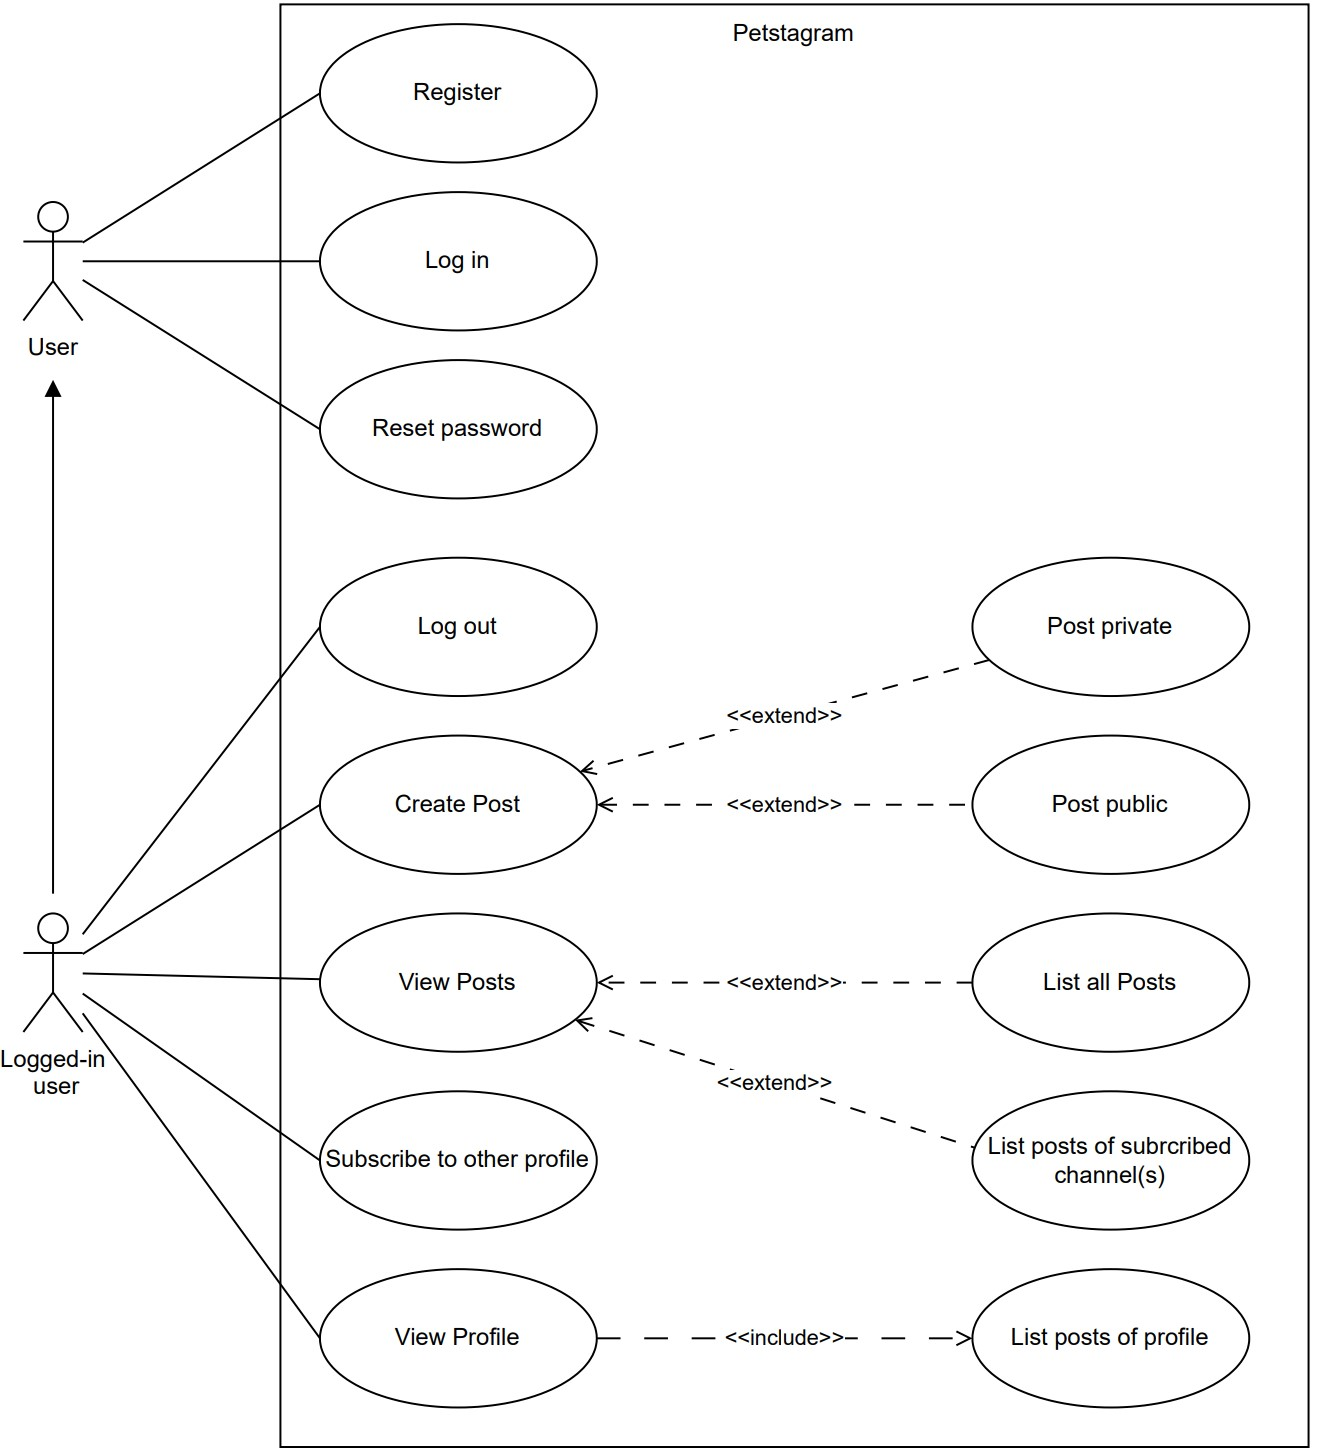
\includegraphics[width=3.5 in]{use-case-diagram}
    \caption{Use Case Diagram}
    \label{fig:fig_use-case-diagram}
\end{figure}

\section{Preliminary or Related Works}
\noindent 
The field of fault tolerance in cloud-based systems has been extensively studied in recent years. In this section, we provide an overview of some key research papers that have contributed to this field, especially with a focus on the topic of load balancing.

The paper "Fault-Tolerance in the Scope of Cloud Computing" \cite{paper_faultTolerance} provides a detailed understanding of fault-tolerance methods required for ensuring high availability and reliability in cloud computing environments. They highlight fault tolerance component and system-level metrics considered in cloud computing. The paper further discusses state-of-the-art proactive and reactive approaches to cloud computing fault tolerance and enumerates future research directions specific to cloud computing fault tolerance development.

Another related work is "A Survey of Fault Tolerance Architecture in Cloud Computing" \cite{paper_surveyArchitectures}. In this paper, the authors examine fault tolerance methods for cloud computing services and outline various policies and methods for implementing fault tolerance in the cloud, including HAProxy. The paper compares various fault tolerance architectures in terms of the type of policy employed in the architecture and the method of fault detection and fault recovery.

The research paper titled "A Comprehensive Study of Load Balancing Approaches in the Cloud Computing Environment and a Novel Fault Tolerance Approach" \cite{study_load_balancing} addresses the challenges of load balancing in cloud computing. The paper discusses various load balancing algorithms and parameters, such as throughput, performance, response time, and fault tolerance, with the aim of improving the efficiency and effectiveness of load balancing in cloud environments. It identifies the limitations of traditional load balancing algorithms and proposes a novel approach that incorporates fault tolerance metrics to address these limitations and enhance load balancing in cloud computing.

Lastly, the paper "Autonomic Fault Tolerance using HAProxy in Cloud Environment" \cite{autonomic_fault_tolerance} explores fault tolerance techniques in cloud computing to enhance server application performance and availability. It highlights the need for fast, reliable, and autonomic fault tolerance systems due to the high level of communication and server failures in cloud environments. The proposed solution utilizes HAProxy, a software tool offering high availability, to handle server failures in virtual machine frameworks. Experimental results demonstrate that HAProxy enables server applications to recover from faults within milliseconds, thereby increasing system availability and reliability.

The existing literature offers valuable insights into various fault tolerance approaches in cloud-based systems and their effects on performance, cost, and complexity. However, a comprehensive analysis and evaluation of these approaches are lacking. This research paper aims to address this gap by building upon the current knowledge base and investigating the latest advancements and trends in fault tolerance strategies. Specifically, the study focuses on comparing the fault tolerance capabilities of Google Cloud's native load balancer with those of HAProxy, considering their performance, cost, and complexity aspects.

\section{Design}
\subsection{Key Design Decisions}
\noindent
Table \ref{table:tbl_Key_Design_Decisions} on page \pageref{table:tbl_Key_Design_Decisions} refers to the Key Design Decisions for our prototypical application.
The prototype "Petstagram" is a web application that incorporates a number of key design decisions across multiple categories, including technology, infrastructure, architecture style, and security. These decisions were made with the aim of creating a highly scalable, reliable, and performant application that can handle large amounts of data and high traffic.

One of the most important technology decisions is the selection of Google Cloud Platform (GCP) as the cloud provider, which offers a cost-effective and scalable infrastructure for hosting and deploying the application. The decision to use a distributed monolith architecture with load balancing ensures high availability and reliability of the system. Additionally, redundancy and fault tolerance mechanisms, such as server replication, data backups, and load balancing, are implemented to ensure that the system can withstand failures and continue to operate.

To address security concerns, SSL/TLS encryption and data encryption are used to protect sensitive user data. Furthermore, caching mechanisms are implemented to improve performance and reduce the load on the database.

One of the key design decisions related to the research question is the implementation of two load balancer approaches, including a software-based HAProxy and a cloud-based Google Cloud Platform Load-Balancing-as-a-Service (LBaaS). This decision enables a comparison of fault tolerance capabilities, performance, cost, and complexity between the two load balancer approaches.


\subsection{System Context}

\noindent Figure \ref{fig:system-context_Component-Diagram} shows a component diagram to describes the system context. 

\begin{figure}[!t]
    \centering
    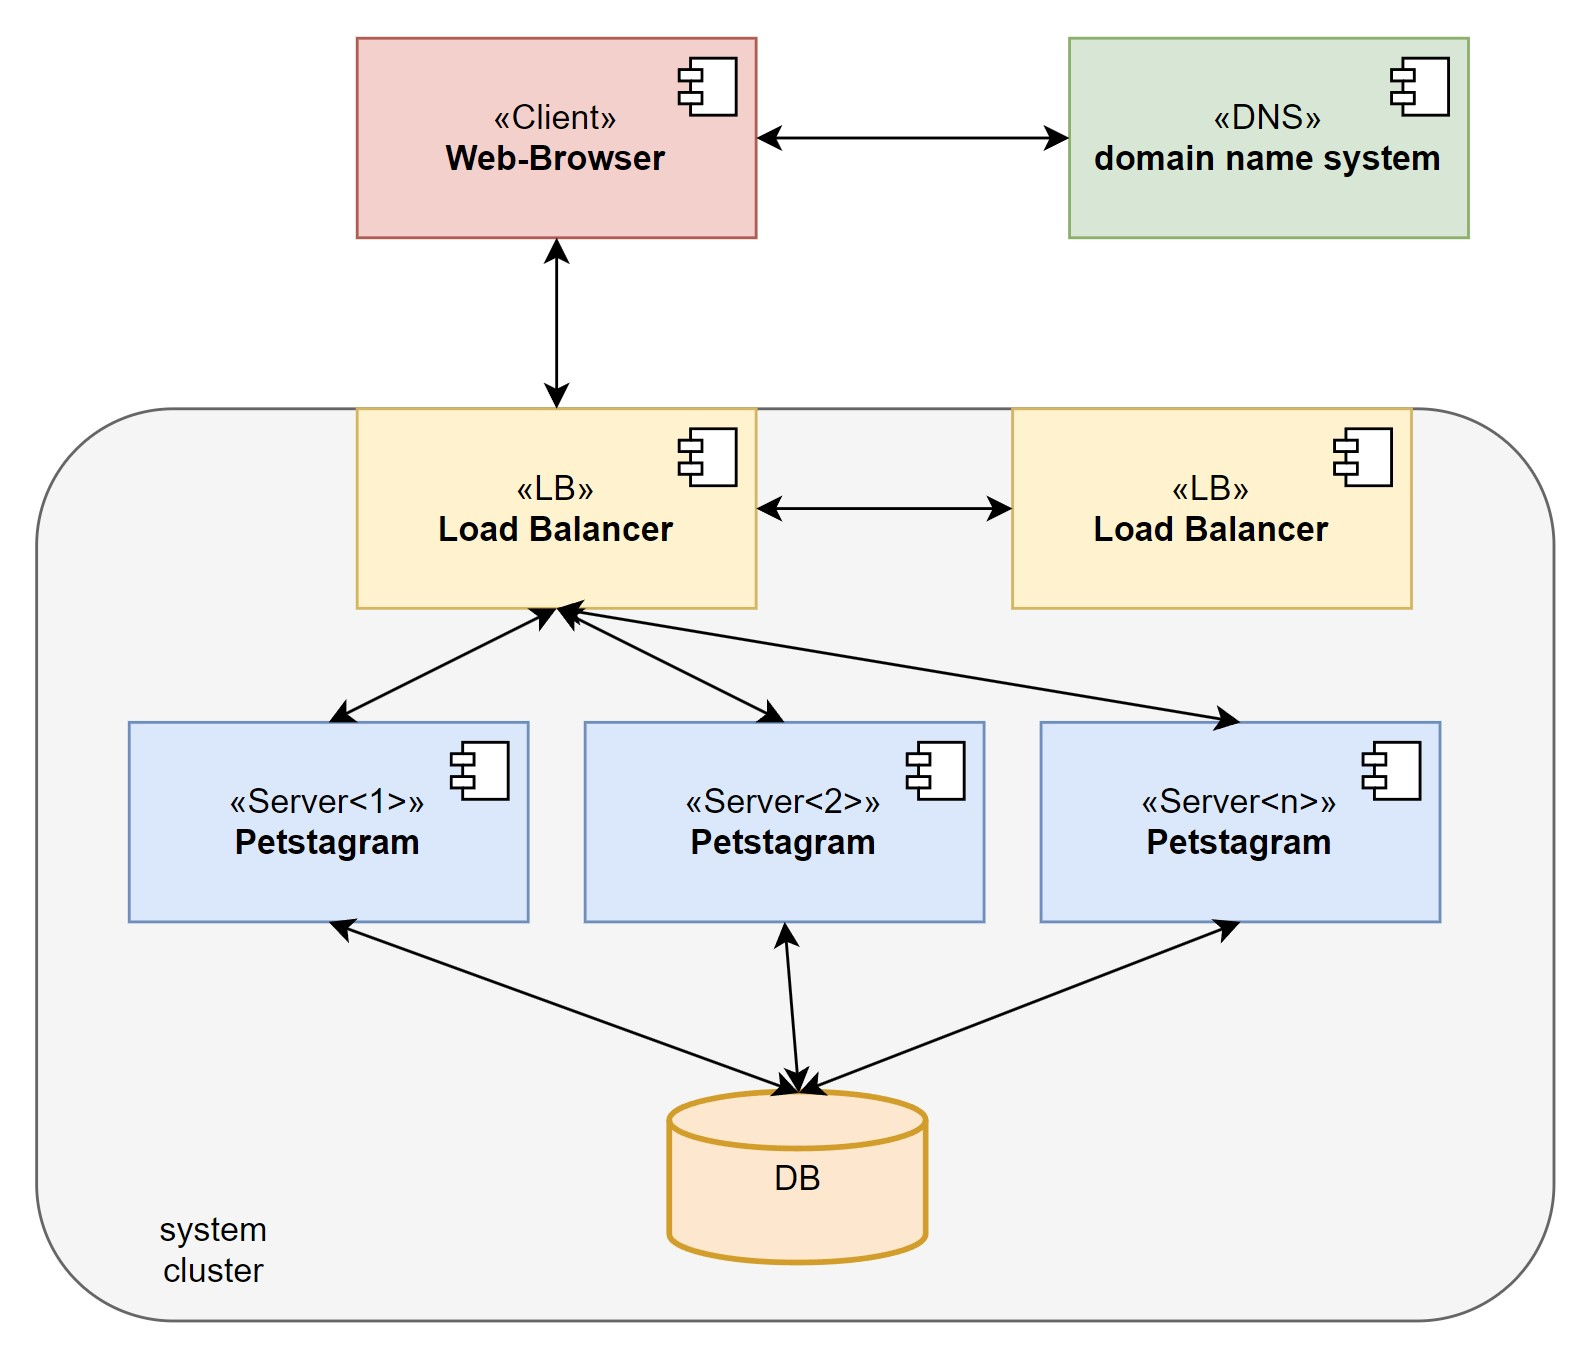
\includegraphics[width=3.5 in]{diagrams/system-context_Component-Diagram}
    \caption{System Context: component diagram}
    \label{fig:system-context_Component-Diagram}
\end{figure}

At the user interface level, the client communicates with the system through a web browser. The client's requests are channeled via a Domain Name System (DNS), which translates human-readable domain names into Internet Protocol (IP) addresses, thereby establishing a seamless and intuitive interface for the user.

The client's requests are then transmitted to a load balancer, a critical component of the architecture that ensures the equitable distribution of network or application traffic across multiple servers. This mechanism mitigates the risk of server overloads, thus optimizing response times and preventing potential service disruptions.

In addition, the load balancer is equipped with a passive counterpart - a secondary load balancer that stands ready to assume control in the event of a failure or disruption in the primary balancer. This failover mechanism enhances the system's resilience and reliability, ensuring uninterrupted service to the users.

The application itself is constructed as a monolithic system, comprising multiple instances distributed across different servers. Each instance is a self-contained component of the system, possessing the ability to operate independently while also contributing to the aggregate functionality of the application.
These instances are all tied to a central database, which acts as the primary repository for all data interactions within the system. 




\subsection{Component View}
\noindent
Petstagram is a web application that will be built using Django \cite{django}, a powerful and popular web framework based on Python. Django provides an intuitive and modular structure that makes it easy to build complex applications quickly and efficiently. One of the key advantages of Django is its ability to handle large amounts of data and traffic, making it a perfect fit for distributed systems like Petstagram.

The external part of the system consists of two components, DB (Database) and MediaCDN (Content Delivery Network). These components are responsible for managing and delivering the data and media content required by the system. The DB component is responsible for storing and managing the data that the system requires. It contains the four main models, which are User, Post, Comment, and Media. These models are the basis for the system's data architecture and provide the necessary information for the system to function correctly.

The MediaCN component is responsible for delivering the media content to the users. It is connected to the Media model, which contains the media data, as well as the Landing and Post views. These views are responsible for displaying the media content, and MediaCDN provides the necessary delivery mechanism.

The Petstagram in the diagram represents the main application logic, which includes the models, views, and templates that define the functionality and appearance of the system. The models include User, Post, Comment, and Media, which define the data used by the application. The views include Authentication, Profile, Landing, and Post, which define the logic used to handle user requests and display information to users. The templates include Auth, Profile, Landing, and Post, which define the layout and appearance of the system.

In addition, the User model is connected to the Authentication view through the Auth template, which is used to display the login form to users. The Post model is connected to the Profile view through the Profile template, which is used to display information about a user's profile. The Comment model is connected to the Landing view through the Auth template, which is used to display the comments section for each post. Finally, the Media model is connected to the Post view through the Post template, which is used to display images and videos associated with each post.

The connections between the components ensure that the necessary information is passed between the models, views, and templates, allowing the system to function correctly. Overall, the Component View diagram provides a clear and concise representation of the various components that make up the Petstagram system and their relationships. It demonstrates how the DB and MediaCDN components work together with the Petstagram application logic to provide a scalable and reliable web application.

\begin{figure}[!t]
    \centering
    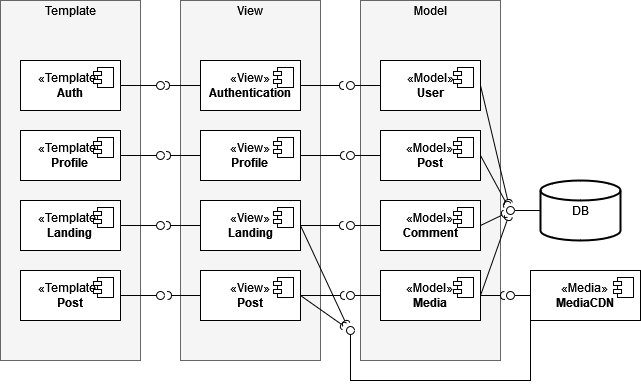
\includegraphics[width=3.5 in]{diagrams/ComponentView.png}
    \caption{component diagram}
    \label{fig:ComponentView}
\end{figure}

\subsection{Data Schema}

\noindent The project's data schema is conceptualized using an Entity-Relationship Diagram (Figure \ref{fig:ERD}), providing a detailed view of the database structure and highlighting the entities, their attributes, and the relationships among them. The ERD serves as a blueprint for our database, outlining how data is stored, organized, and manipulated.

The User table is holding all details related to a user's account. It comprises of "user\_id", "name", "password", "description", and "email". The "user\_id" serves as a unique identifier for each user, enabling a connection to other tables. 

The Post table stores all posts generated by users. Each post is identified by a unique "post\_id", with a "user\_id" field linking it to the respective user who made the post. "Likes" indicates the popularity of the post, "description" provides a summary, "date" records when the post was made, and "media\_id" ties the post to any associated media in the Media table. 

The Media table acts as a repository for all media assets shared across the platform. Every media item possesses a unique "media\_id" and an "url", which points to the online location of the media item. 

Lastly, the Comment table stores all comments made by users on posts. Each comment is identified by a unique "commend\_id" and has an "order\_id" for sequencing, "poster\_id" to link it to the user who posted it, "text" for the comment's content, and "date" to timestamp when the comment was posted.





\begin{figure}[!t]
    \centering
    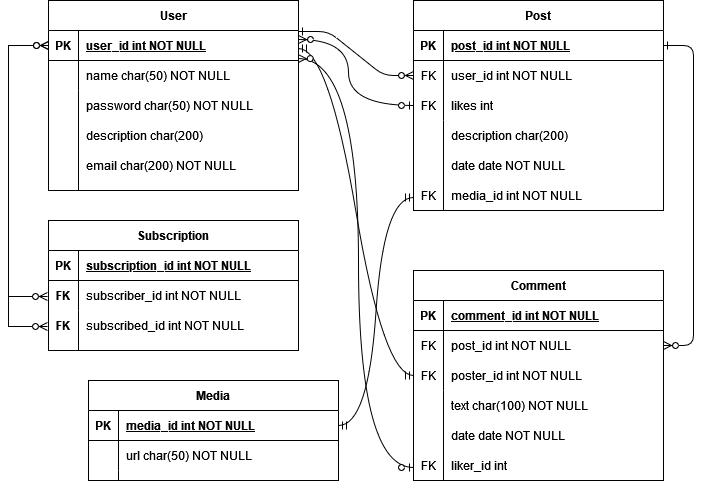
\includegraphics[width=3.5 in]{diagrams/ERD}
    \caption{Entity relationship diagram of the system}
    \label{fig:ERD}
\end{figure}

\noindent

\subsection{Runtime View}
\noindent
As figure \ref{fig:fig_use-case-diagram} on page \pageref{fig:fig_use-case-diagram} shows, important use-cases of Petstagram are the display and creation of posts. Petstagram is accessed via REST API HTTP requests. Figure \ref{fig:createPost} shows the sequence diagram for the creation of a post object. The user sends a POST HTTP request via the client to the server, the Django view class handles the POST request and saves the new post model with the data send by the user. The client receives a HTTP 201 response. 
\begin{figure}[!t]
    \centering
    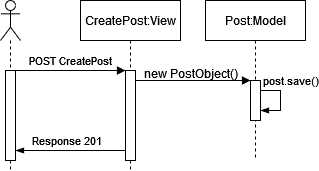
\includegraphics[width=3.5 in]{diagrams/createPost_sequence.drawio.png}
    \caption{createPost sequence diagram}
    \label{fig:createPost}
\end{figure}

Figure \ref{fig:viewProfile} shows the sequence for the display of a profile. The client send a GET HTTP request with the id of the profile to the view class. The class gets the user object from the database and sends it back to the client.

\begin{figure}[!t]
    \centering
    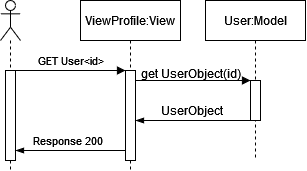
\includegraphics[width=3.5 in]{diagrams/viewProfile_sequence.drawio.png}
    \caption{viewProfile sequence diagram}
    \label{fig:viewProfile}
\end{figure}

Figure \ref{fig:listPosts} shows the sequence for the display of the content feed, which acts as the index page for all users. The client sends a GET requests, the view gets the ID of the user and gets a the posts of all users which are subscribed. The posts are returned in a HTTP 200 response.

The Django web framework allows a straight logic, where the view accesses the database through the model.
\begin{figure}[!t]
    \centering
    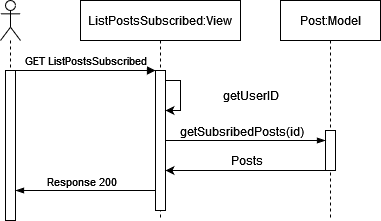
\includegraphics[width=3.5 in]{diagrams/ListPostsSubscribed_sequence.drawio.png}
    \caption{listPosts sequence diagram}
    \label{fig:listPosts}
\end{figure}

\subsection{Crosscutting Concepts}
\noindent
In the previous chapters, we discussed the architecture of Petstagram. We aim to compare the fault tolerance capabilities of Google Cloud's native load balancer and HAProxy. To achieve this, this chapter will describe several important crosscutting concepts that are integral to the Petstagram web application. These concepts cannot be fully accommodated in the previous chapters, as they relate to overarching design and infrastructure considerations that affect the entire system. The following table \ref{table:tbl_Crosscutting_Conceptss} on page \pageref{table:tbl_Crosscutting_Conceptss} summarizes the key crosscutting concepts, including a brief explanation of each concept and its rationale:

Petstagram leverages horizontal and vertical scaling through auto-scaling capabilities provided by the Google Cloud Platform to address scalability challenges. Using health checks to monitor the availability and performance of the web servers is an essential aspect of the Petstagram system, as it ensures that the load balancer can accurately distribute traffic and maintain the overall stability and reliability of the system. Petstagram uses database sharding to partition data into smaller subsets that can be stored across multiple servers to improve performance and scalability. Content Delivery Network (CDN) \cite{google_cdn} and load balancing provided by the Google Cloud Platform and HAProxy are employed to optimize the application's performance, distribute traffic, and minimize the risk of downtime. The development process uses continuous integration and deployment (CI/CD) to automatically build, test, and deploy code changes to production. For this, the application is hosted on an internal GitLab instance. The architecture supports SSL/TLS encryption, internationalization, and employs the Model-View-Template (MVT) pattern. Additionally, unit testing is employed to improve code quality.

In conclusion, the crosscutting concepts presented in this chapter are crucial for ensuring the scalability, performance, maintainability, security, and user experience of the Petstagram web application. By incorporating these concepts into the architecture, Petstagram can be designed to handle increasing user demand, provide a seamless user experience, and improve overall reliability.

\clearpage
\newpage
% \pagebreak
\begin{thebibliography}{1}
\bibliographystyle{IEEEtran}
%\bibliography{references}
\bibitem{cloud_demand} Public cloud application services/software as a service (SaaS) end-user spending worldwide from 2015 to 2024 (in billion U.S. dollars) [Graph], Gartner, April 19, 2023. [Online]. Available: https://www.statista.com/statistics/505243/worldwide-software-as-a-service-revenue/ (accessed May 09, 2023).
\bibitem{load_balancing} AWS Amazon, "What Is Load Balancing?," Accessed: May. 09, 2023, [Online]. Available: https://aws.amazon.com/what-is/load-balancing
\bibitem{gce_load_balancer} “Load Balancing” Google LLC, 2023. https://cloud.google.com/load-balancing (accessed May 16, 2023).
\bibitem{haproxy} “HAProxy - The Reliable, High Perf. TCP/HTTP Load Balancer,” www.haproxy.org. https://www.haproxy.org (accessed May 16, 2023).
\bibitem{about_HAProxy} HAProxy, "HAProxy Enterprise," Accessed: May. 09, 2023, [Online]. Available: haproxy.com/products/haproxy-enterprise
\bibitem{about_Cloud_Load_Balancing} Google Cloud, "Cloud Load Balancing overview," Accessed: May. 09, 2023, [Online]. Available: https://cloud.google.com/load-balancing/docs/load-balancing-overview
\bibitem{paper_faultTolerance}
A. U. Rehman, R. L. Aguiar, and J. P. Barraca, “Fault-Tolerance in the Scope of Cloud Computing,” IEEE Access, vol. 10, 2022, doi: https://doi.org/10.1109/ACCESS.2022.3182211.
\bibitem{paper_surveyArchitectures} M. Nazari Cheraghlou, A. Khadem-Zadeh, and M. Haghparast, “A survey of fault tolerance architecture in cloud computing,” Journal of Network and Computer Applications, vol. 61, pp. 81–92, Feb. 2016, doi: https://doi.org/10.1016/j.jnca.2015.10.004.
\bibitem{study_load_balancing}M. A. Shahid, N. Islam, M. M. Alam, M. M. Su’ud, and S. Musa, “A Comprehensive Study of Load Balancing Approaches in the Cloud Computing Environment and a Novel Fault Tolerance Approach,” IEEE Access, vol. 8, pp. 130500–130526, 2020, doi: 10.1109/ACCESS.2020.3009184.
\bibitem{autonomic_fault_tolerance} V. Kaushal and A. Bala, “Autonomic fault tolerance using HAproxy in cloud environment,” Int. J. of Advanced Engineering Sciences and Technologies, vol. 7, no. 2, pp. 54–59, 2011.
\bibitem{django} “Django - DjangoThe web framework for perfectionists with deadlines.,” Django Project, https://www.djangoproject.com/ (accessed May 16, 2023). 
\bibitem{google_cdn} “Cloud CDN,” Google LLC, https://cloud.google.com/ (accessed May 16, 2023).


\end{thebibliography}
\clearpage
\newpage
\appendix
\section{Key Design Decisions}\label{appendix:key_design_decisions}
\begin{table}[htpb]
    \caption{Key Design Decisions.}
    \label{table:tbl_Key_Design_Decisions} 
    \begin{tabular}{ |m{3cm}|m{2cm}|m{11cm}| } 
        \hline
        Decision&Category&Explanation\\
        \hline
        Django python web framework&technology&Django is a highly scalable web framework with a robust set of features and an active community. It provides a Model-View-Template (MVT) architecture, built-in admin interface, and support for database ORM. Django's scalability is an essential feature for Petstagram since it can handle large amounts of data and high traffic.\\
        \hline
        PostgreSQL &technology&PostgreSQL is a widely-used and robust relational database management system that is known for its scalability, reliability, and performance. It has excellent support for ACID (Atomicity, Consistency, Isolation and Durability) transactions and provides features such as stored procedures and triggers that can be useful in complex applications like Petstagram.\\
        \hline
        Google Cloud Platform&technology&Google Cloud provides a robust, reliable, and scalable platform for hosting and deploying web applications like Petstagram. It also offers a native Load Balancer service, which is to be used in the course of the comparison.\\
        \hline
        Distributed monolith&architecture style&Petstagram will be implemented as a distributed monolith architecture. The server can be replicated to provide scalability, and the requests to the system will be handled by a load balancer, which balances the load to the multiple servers. This architecture style can help ensure reliability and high availability. Furthermore, Petstagram offers only a few services and focuses on providing the main functionalities, which is why a subdivision into microservices does not make sense. A monolithic application enables easier deployment and also facilitates debugging.\\
        \hline
        Non-distributed database&technology&Petstagram will use a non-distributed database, meaning that there will be only one primary database instance that is responsible for handling all the database operations. This approach can simplify the database design and reduce complexity and avoids synchronizing the data on different data nodes.\\
        \hline
        Cloud Storage&infrastructure&Petstagram will use cloud storage to store user-uploaded images and media files. This allows for scalability and easy access to data from anywhere in the world.\\
        \hline
        Browser as a client&organizational&Petstagram will use a browser as the client application, meaning that the application will be accessed through a web browser. This approach can provide ease of use, accessibility, and platform independence.\\
        \hline
        Redundancy and Fault Tolerance&quality&Petstagram will implement redundancy and fault tolerance mechanisms to ensure that the system can withstand failures and continue to operate. These mechanisms include replication of servers, data backups, and load balancing.\\
        \hline
        Caching&quality&Petstagram will implement caching mechanisms to improve performance and reduce the load on the database, such as using a caching layer like Redis or Memcached.\\
        \hline
        Cloud Deployment&infrastructure&Petstagram will be deployed on the cloud platform Google Cloud Platform (GCP), which provides a cost-effective and scalable infrastructure. This approach can help reduce hardware and software maintenance costs, increase flexibility, and ensure high availability. In addition, this cloud provider guarantees a high level of security, which is of significant importance when dealing with customer data.\\
        \hline
        Load Balancer&infrastructure&Due to an expected high traffic and to ensure/determine proper and cost-efficient distribution, two load balancer approaches will be implemented that can distribute the incoming traffic among multiple servers. One approach will be software-based (HAProxy), the other cloud-based (Google Cloud Platforms Load-Balancing-as-a-Service LBaaS).\\
        \hline
        Data Encryption&security&Petstagram will encrypt sensitive data such as user credentials and personal information in transit and at rest. Data encryption will be implemented using industry-standard encryption algorithms and protocols, such as Advanced Encryption Standard (AES) and Transport Layer Security (TLS). Encrypting sensitive data can help prevent data breaches and unauthorized access to sensitive information.\\
        \hline

    \end{tabular}
    \\
\end{table}

\newpage
\clearpage
\begin{table}[htbp]
    \caption{Crosscutting concepts.}
    \label{table:tbl_Crosscutting_Conceptss} 
    \centering
    \begin{tabular}{ |m{3cm}|m{2cm}|m{11cm}| } 
        \hline
        Crosscutting Concept&Category&Explanation and rationale\\
        \hline
        Scalability&Performance&Petstagram is a web application that may experience spikes in traffic due to user activity. To handle this load, the application should be able to scale horizontally by adding more application servers as needed. In addition, the application should be able to scale vertically by increasing the resources available to each server. This scalability can be achieved auto-scaling as provided by the Google Cloud Platform.\\
        \hline
       Health checks&Operations&Health checks are important for monitoring the availability of the distributed web servers in Petstagram. By performing regular health checks, the load balancer can ensure that only healthy servers are used to handle incoming requests. Health checks can also be used to trigger automatic scaling based on server utilization or to alert operators of potential issues before they become critical.
\\
        \hline
        Model-View-Template (MVT) pattern&design patterns&Petstagram uses the MVT pattern, which separates concerns and helps to maintain code clarity and reusability. The model represents the data and business logic, the view is responsible for presenting the data to the user, and the template is responsible for rendering HTML.\\
        \hline
        Internationalization (i18n)&user experience&Internationalization is supported by using Django's built-in localization framework, allowing the application to be easily translated to support multiple languages. Additionally, the Google Cloud Translation API can be used to automatically translate text content, providing a seamless experience for users in different regions.\\
        \hline
        Content Delivery Network&Performance&Images uploaded by users to Petstagram are stored in a Content Delivery Network (CDN) via Cloud Storage. A CDN is a network of servers that cache and deliver content to users from the server closest to them, reducing the time it takes for users to load content. This can significantly improve the application's performance, especially for users distributed around the world.\\
        \hline
        Database sharding&Data management&Petstagram uses a single PostgreSQL database to store all user data. As the application grows, this may become a bottleneck. One approach to addressing this is to shard the database, which involves partitioning the data into smaller subsets that can be stored across multiple servers. This approach can improve performance and scalability by reducing the load on any single server.\\
        \hline
        Continuous Integration and Deployment&Development&Petstagram is developed using the Django framework, which supports Continuous Integration and Deployment (CI/CD). CI/CD involves automatically building, testing, and deploying code changes to production as soon as they are committed to the source code repository. This approach can improve the application's quality and reliability, while simultaneously simplifying development.\\
        \hline
        Source code repository&Development&Petstagram’s source code is versioned in a single Git repository hosted on the internal GitLab XXXX server.\\
        \hline
        Logging and Monitoring&Operations&Petstagram should be monitored using a logging and monitoring tool. This can provide insights into the application's performance, availability, and errors, allowing developers and operators to identify and fix issues quickly. \\
        \hline
        Unit testing&Testing&Petstagram employs unit testing to ensure that individual components of the system are working as intended. This helps to find bugs early in development and improve code quality.\\
        \hline
        SSL/TLS Encryption&security&Petstagram will use SSL/TLS encryption to ensure secure communication between the client and the server and protect sensitive user data.\\
        \hline
    \end{tabular}
    \\
\end{table}

% \chapter{Second}
% This is my Second Appendix .

\vfill

\end{document}
